%% part4
\MinParskip{}

\subsection{The Optimized Entropy Weight Method (EWM) }
We use the Entropy Weight Method (EWM) to get the weight of indicators. The Entropy Weight Method is an object weighting method, which uses the information entropy idea for reference. It is used to determine the relative weights of different criteria in a decision-making process. It determines the weight of the indicators by calculating the information entropy of the index, according to the impact of the relative change of the index on the overall system.

In other words, the weight of each indicator is given according to the difference degree of the indicator value, and the corresponding weight of each indicator is obtained. The indicator with relatively large change degree has larger weight. 

The greater the entropy, the more chaotic the system is, the less information it carries and the less weight it has. Otherwise, the higher the entropy, the more orderly the system is, the more information it carries, and the greater the weight is.

The first step of the Entropy Weight Method is the standardization of measured values. The standardized value of the jth index in the ith sample is denoted as $p_{ij}$, and its calculation method is as follows:$$p_{ij}=\frac{a_{ij}}{\sum_{i=1}^na_{ij}},i=1,2\cdots,,9,j=1,2,\cdots,9$$

Secondly, in the EWM, the entropy value $e_i$ of the jth index is defined as:$$e_j=-\frac{1}{ln(9)}\sum_{i=1}^np_{ij}ln(p_{ij}),j=1,2,\cdots,9$$

The range of entropy value $e_j$ is [0, 1]. The larger the $e_j$ is, the greater the differentiation degree of index j is, and more information can be derived. Hence, higher weight should be given to the index. 

Therefore, in the traditional EWM, the calculation method of weight is:$$w_j=\frac{1-e_j}{\sum_{j=1}^me_j},j=1,2,\cdots,9$$

It can be seen from the above equation that when $e_j\rightarrow1$,the difference in the entropy value of different evaluation indexes is small, but the difference in the entropy weight is large. Therefore, we use the following equation to calculate entropy weight instead of traditional equation.

$$w_j^{'}=\frac{1+e_j+\sum_{k=1}^ne_k}{\sum_{l=1}^n(1-2e_l+\sum_{k=1}^ne_k)}$$

In the above method, the different entropy weights for different indicators (e.g. $p$ and $q$)become $$\Delta w=2\Delta e/C$$ where $$\Delta e=e_p-e_q,C=\sum_{l=1}^n(1-2e_l+\sum_{k=1}^ne_k)$$

It indicates that the entropy value changes slightly, and its corresponding entropy weight also changes slightly. For the factor with equivalent useful information, the weight information is consistent with the corresponding entropy level.


\begin{table}[H] \centering
    \caption{Weights of the Indicators Calculated from optimized EWM method}
    \begin{tabular}{ccl}
        \toprule
        Indicators & Weights\\ \hline
        All industry total & 0.12709\\
        All tertiary industry percentage & 0.12376\\
        Population Density & 0.12742\\
        Limiting Magnitude & 0.12390\\
        Last Bus Time & 0.12436\\
        Power Consumption per Capita per Month & 0.12378\\
        Annual Precipitation(in millimetre) & 0.12411\\
        Working hours per Week & 0.12581\\
        Nightlife index & 0.12402\\
        \bottomrule
    \end{tabular}
\end{table}


\subsection{The TOPSIS Method}

The Technique for Order of Preference by Similarity to Ideal Solution (TOPSIS) is a multi-criteria decision-making method that is used to determine the best option from a set of alternatives based on multiple criteria. 

First of all, we use Min-Max normalization to process the data.

For the benefit-attributed data,
$$b_{ij}=\frac{a_{ij}-a_j^{min}}{a_j^{max}-a_j^{min}}$$

And for the cost-attributed data,
$$b_{ij}=\frac{a_{j}^{max}-a_{ij}}{a_j^{max}-a_j^{min}}$$

All these data form the normalized matrix $B$. We then multiply each value in a column with the corresponding weight given, and get weighted-normalised decision matrix, which $$C=W*B$$

Secondly, calculating the positive ideal solution $C^*$ and the negative ideal solution $C_0$, which$$C^*=[b_1^{max},b_2^{max},\cdots,b_8^{max}]$$ $$C_0=[b_1^{min},b_2^{min},\cdots,b_8^{min}]$$

Now we need to calculate Euclidean distance $s_i^{0}$ for elements in all rows from the positive ideal solution and the negative ideal solution.$$s_i^{0}=\sqrt{\sum_{i=1}^{3}(b_{ij}-C_i^{*})^{2}},j=1,2\cdots,9$$

Here, $s_i^*$ is the best distance calculated on the i-th row, where $b_{ij}$ is element value and $C_i^{*}$ is the ideal best for that column. Similarly, we can find $s_i^0$, which is the worst distance calculated on the i-th row.

Finally, calculate the TOPSIS Score and Ranking. For $C_i,i=1,2,\cdots,9$, solve $s_i^*$, the distance to the positive ideal solution $C^*$, and $s_i^0$, the distance to the negative ideal solution $C_0$

Now that we have $s_i^*$ and $s_i^0$. Then calculate the Topsis score for each row, and get the final score and ranking. $$f_i=\frac{s_i^0}{s_i^*+s_i^0}$$

\subsection{Application of the Model on the Four Locations}


\subsubsection{A Protected Land Location: Wyoming}
For a protected land location, we choose Wyoming. Wyoming is a state in the Mountain West subregion of the Western United States. Almost half of the land in Wyoming is owned by the federal government, generally protected for public uses.

Wyoming is the least populous state despite being the 10th largest by area, with the second-lowest population density after Alaska. And it's population density is 5.9 men per $km^2$. Since the sparse population, it's GDP is only 41510.2 million dollars per year. Without much demand for transportation, it's local bus deadline is 5 p.m., which largely reduce it's demand for road illumination. The nightlife index is only 37, which reason is closely related to the indicators above. This may account for the low power consumption, which is only 128.9 kWh. 

Today, Wyoming's economy is largely based on tourism. So its tertiary industry percentage of GDP is similar to New York, which is one of the most prosperous city in the world. And the detailed data for tertiary industry percentage of GDP is 0.247. To support it's tourism, people should work for more hours, so we can see it's working hour is 40.3 hours per week.

Due to it's geographical position, it's annual precipitation is 390 millimeters. And with its vast land, the limiting magnitude in Wyoming is 8.3, which means you can see several faint planet.

According to the indicators we mentioned before, it's night-light intensity score in our model is 0.18786, which ranks the lowest in our selected locations. This shows that our model's application for protected location is in line with the reality.
\begin{figure}[H]\centering
    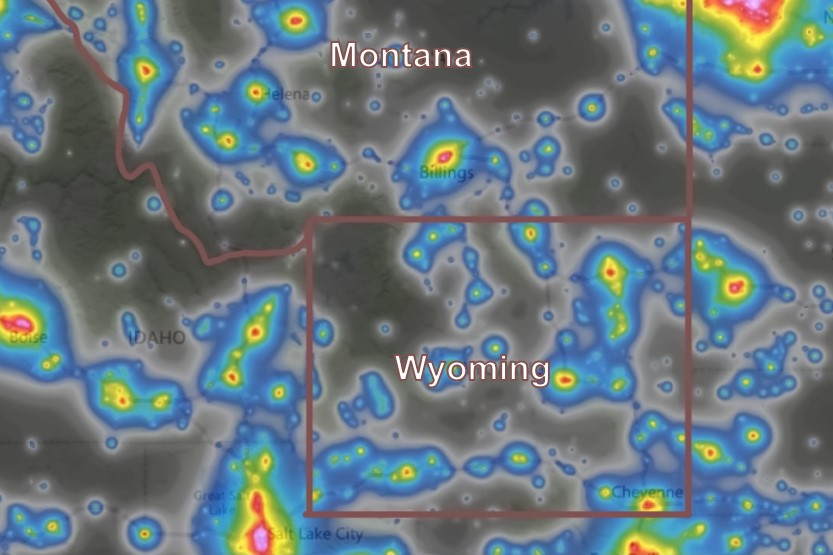
\includegraphics[width=0.9\textwidth]{figures/texted/Wyoming_new.jpg}
    \caption{Night-time Light Intensity of Wyoming} \label{fig:figure3}
\end{figure}


\subsubsection{A Rural Community: Nevada}
For a rural community, we choose Nevada. Nevada is the 7th-most extensive, the 32nd-most populous, and the 9th-least densely populated of the US states. Its population density is 28.3 men per $km^2$. And its working hour belongs to the average level in US.

As we all know, Las Vegas is located in Nevada. This may account for its night-life index of up to 70.Nevada's power consumption is 362.8 kWh per month, far more than protected locations, but similar to other locations.

Legalized gambling and lenient marriage and divorce laws transformed Nevada into a major tourist destination in the 20th century, which promote local economy. Its GDP is 194486.6 per year and its tertiary industry percentage of GDP is 0.284. The early deadline of bus is mainly because of tourism. Its local bus deadline is 3 p.m.

Nevada is the driest state, and its annual precipitation is 241 millimeters. Its limiting magnitude is 8.3, which means you can rarely see faint planet.

According to the indicators we mentioned before, its night-light intensity score in our model is 0.38081, which ranks above all the protected locations in our selected locations, but below all the more prosperous states. This shows that our model's application for rural community is in line with the reality.

\subsubsection{A Suburban Community: California}
Although California is full of modern metropolises such as Los Angeles and San Fransisco, we categorize it as a suburban community, since most area of California is not cities but suburban areas and hilly areas.

California is the third-largest state by area, and more than this, it also has a high population density of 253.7 men per $km^2$, resulting in the most populated state in the U.S.

Due to its huge population, the economy of California is no doubt the largest in the United States. Its GDP is 3373240.7 per year, far more than any other state, and it's night-life index is 65. It's working hour is 38.3 hours per week, similar to other states.

Sacramento is the state's capital, while Los Angeles is the most populous city in the state and the second most populous city in the country. So it has the highest power consumption among suburban communities, which values 394.2. And it also has the latest deadline of local bus, which is 11:30 p.m.

California has a Mediterranean climate, depending on latitude, elevation, and proximity to the Pacific Coast. Its terrain varies widely from hot desert to alpine tundra. The average annual precipitation is 563 millimeters. And its limiting magnitude is 6, which means it's hard for you to see the stars by eyes.

According to the indicators we mentioned before, its night-light intensity score in our model is 0.59146, highest in the suburban locations, but lower than Massachusetts and New York. It clearly reflects the high density of the suburban regions of California, and the result is in line with the reality.

\begin{figure}[H]\centering
    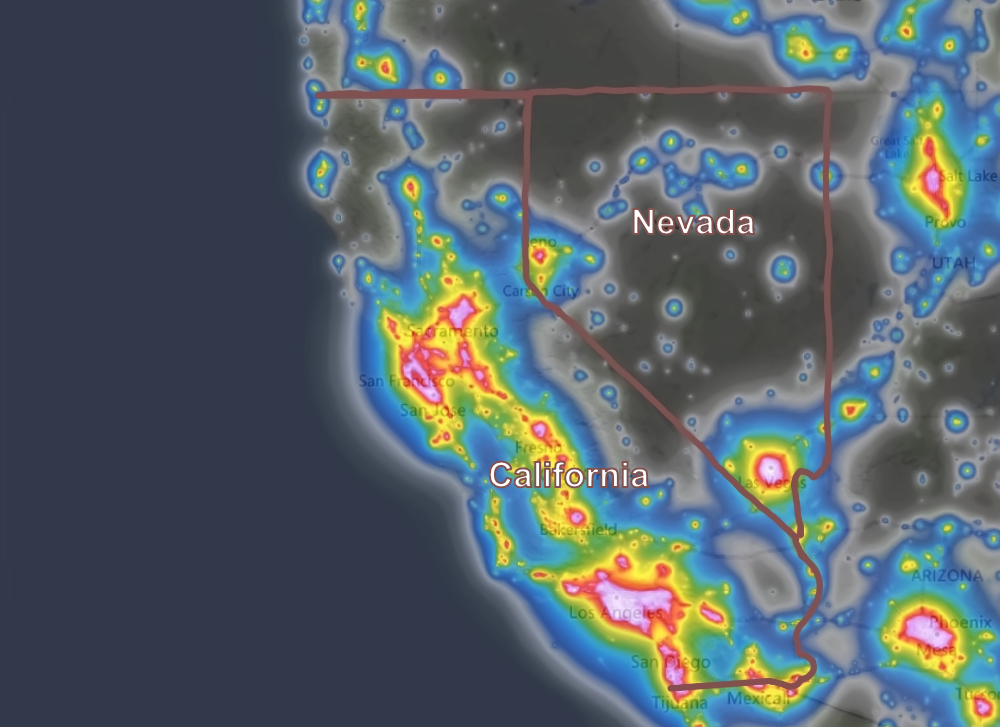
\includegraphics[width=0.9\textwidth]{figures/texted/Nevada.jpg}
    \caption{Night-time Light Intensity of California and Nevada} \label{fig:figure4}
\end{figure}


\subsubsection{An Urban Community: New York}
New York State is a highly developed state with a world famous international metropolis, New York. State of New York was one of the original Thirteen Colonies forming the United States. With a total area of 54,556 square miles (141,300 $km^2$), New York is the 27th-largest U.S. state by area. But also, it is the fourth-most-populous state in the United States as of 2021, with 20.2 million people.

Due to its great importance in USA's and international economy, it's GDP is 1901296.5 million dollars per year. And in serving its highly developed service industry, it's local bus deadline is 1 a.m, and the nightlife index is 83, ranks the top of the chosen locations. And this leads to a huge power consumption, which is 412.8 kWh. 

Since New York is famous for its economy, its tertiary industry percentage is the highest among the chosen locations. And it seems that people in New York States enjoys their life, as their average working hour is 38.4 hours per week.

New York State has a temperate continental humid climate, with an annual precipitation 1062 millimeters. And with its well-explored land, the limiting magnitude in New York State is 4, which means you can seldom see faint planets.

According to the model, New York State night-light intensity score is 0.69031, which ranks the highest in all, in line with the reality.

\begin{figure}[H]\centering
    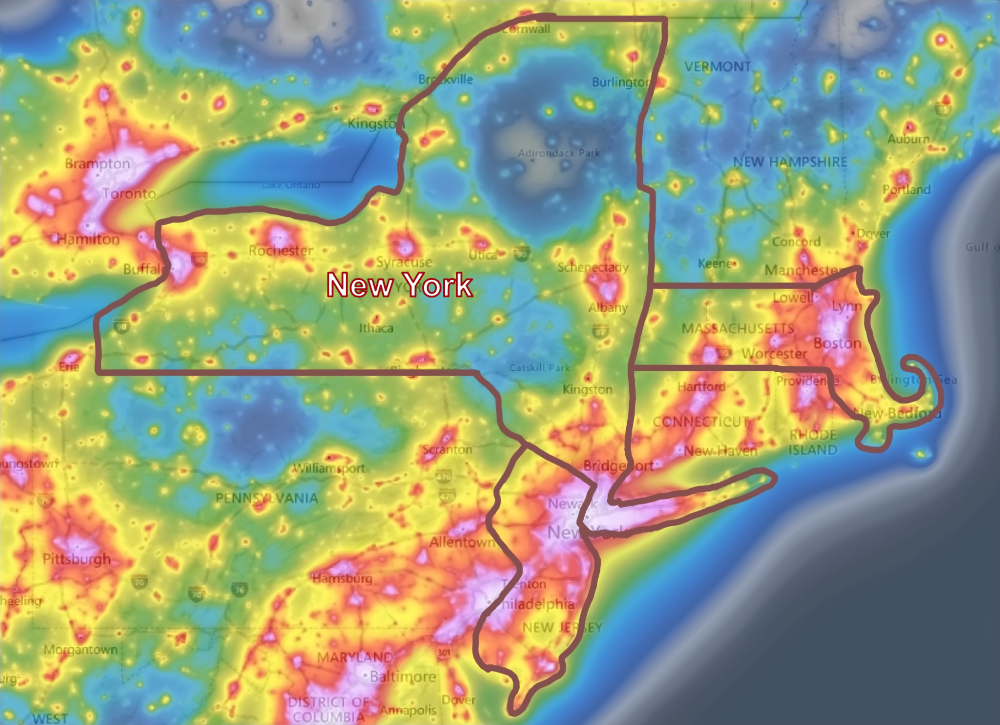
\includegraphics[width=0.9\textwidth]{figures/texted/New_York.jpg}
    \caption{Night-time Light Intensity of New York State} \label{fig:figure5}
\end{figure}

\subsubsection{Result of the TOPSIS Score and Ranking}

\begin{table}[H] \centering
    \caption{Result of the TOPSIS Score and Ranking}
    \begin{tabular}{llll}
        \toprule
        Types of Locations & States & Score & Ranking\\ \hline\hline
        \multirow{3}{*}{\textbf{Urban Communities}}& New York & 0.69031 & \multicolumn{1}{c}{1}\\
                            &  Massachusetts & 0.60754 & \multicolumn{1}{c}{2}\\
                            & New Jersey & 0.59492& \multicolumn{1}{c}{3}\\\hline
        \multirow{3}{*}{\textbf{Suburban Communities}} & California & 0.59146 & \multicolumn{1}{c}{4}\\
                            & Pennsylvania & 0.48859 & \multicolumn{1}{c}{5}\\
                           & Washington & 0.40662 & \multicolumn{1}{c}{6}\\\hline
        \multirow{3}{*}{\textbf{Rural Communities}}& Missouri & 0.40527 &\multicolumn{1}{c}{7}\\
                            & Nevada & 0.38081 & \multicolumn{1}{c}{8}\\
                            & Mississippi & 0.36775 & \multicolumn{1}{c}{9}\\\hline
        \multirow{3}{*}{\textbf{Protected Land Locations}}& Montana & 0.34936 & \multicolumn{1}{c}{10}\\
                            & Alaska & 0.21363  & \multicolumn{1}{c}{11}\\
                           & Wyoming & 0.18786 & \multicolumn{1}{c}{12}\\
        \bottomrule
    \end{tabular}
\end{table}

\begin{figure}[H]\centering
    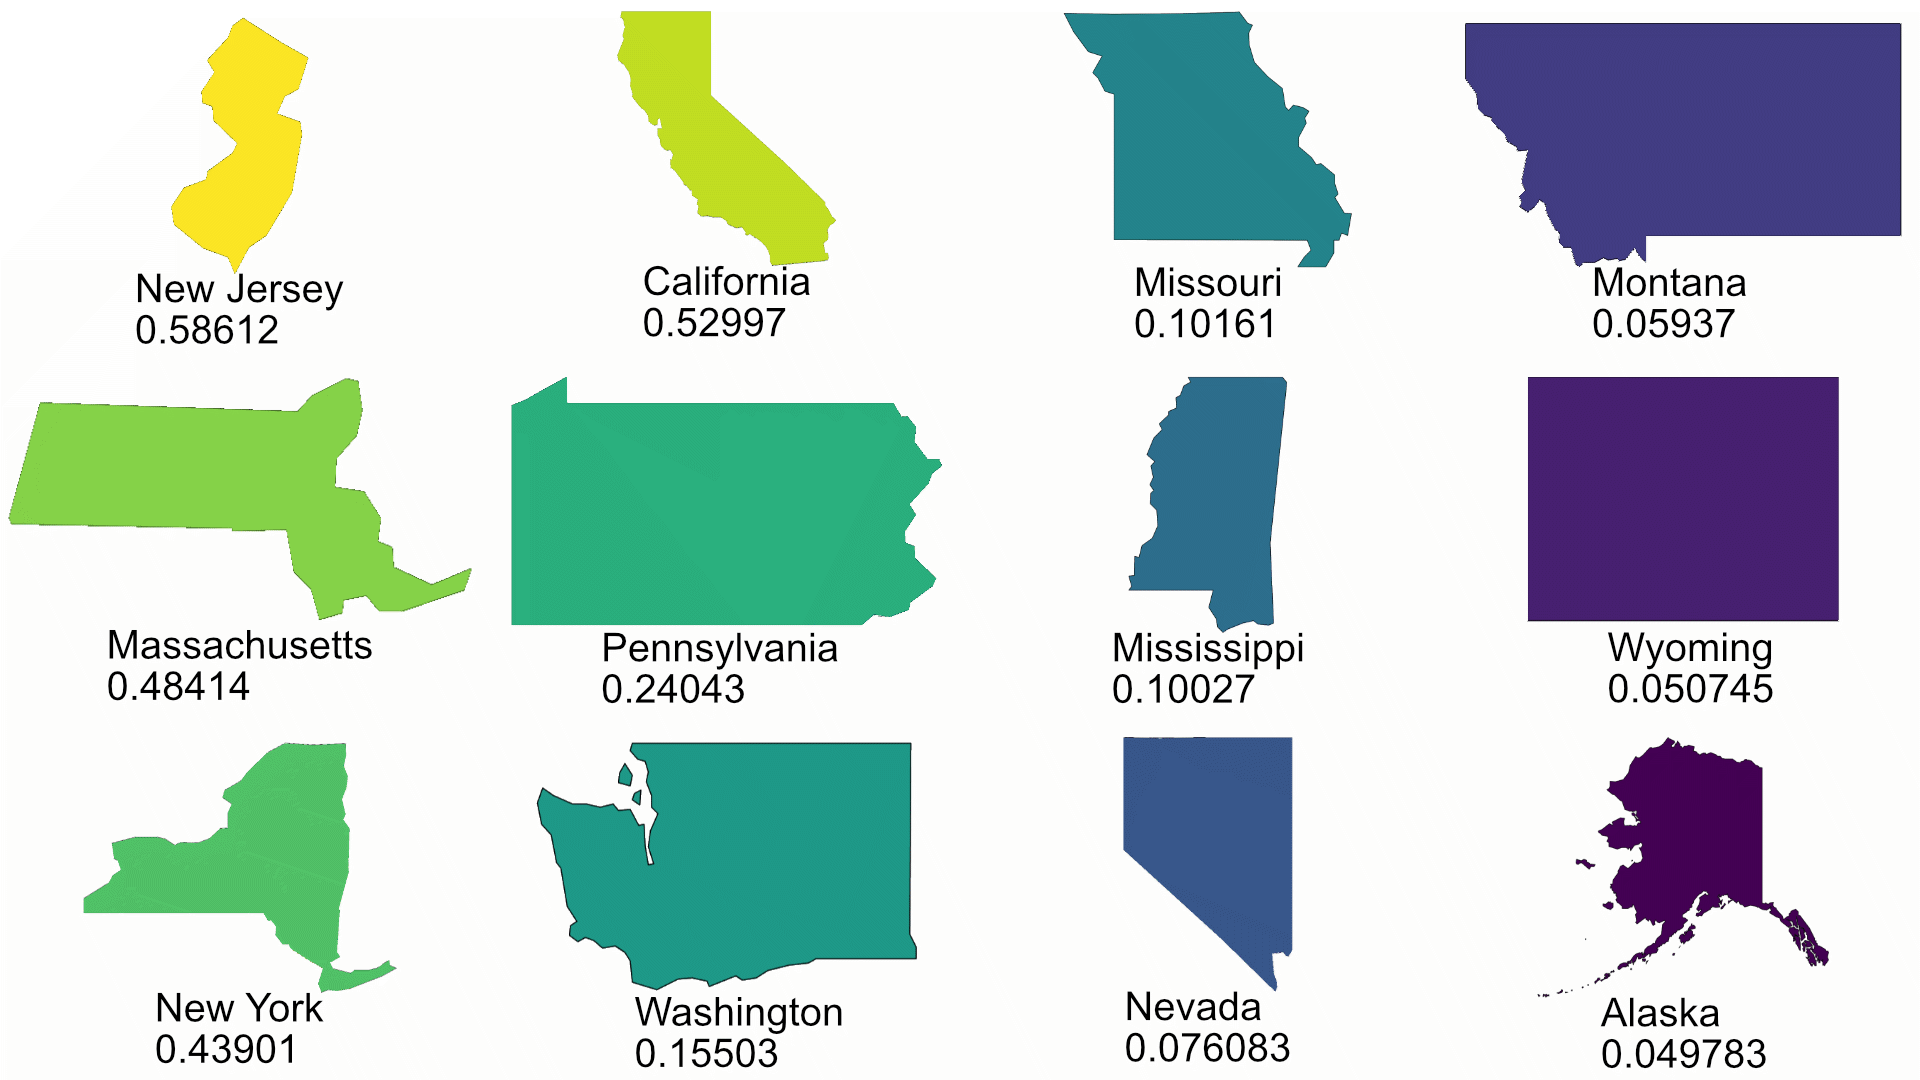
\includegraphics[width=1\textwidth]{figures/result.png}
    \caption{Result of the TOPSIS Score and Ranking} \label{fig:figure6}
\end{figure}